%%
%%  chapter01.tex - Obstacle Detection and Planning for Autonomous Vehicles based on Computer Vision Techniques
%%
%%  Copyright 2014 Néstor Morales <nestor@isaatc.ull.es>
%%
%%  This work is licensed under a Creative Commons Attribution 4.0 International License.
%%

\graphicspath{{./images/chapter01/bmps/}{./images/chapter01/vects/}{./images/chapter01/}}

\chapter{Problem Statement and Previous Work}\label{ch:chapter01}

\section{Problem Statement}\label{ch:chapter01_01}

Computer Vision environment understanding targeted at enabling autonomous operation of a robotic platform has been widely studied over the years, leading to the creation of some prototype vehicles \cite{Maurer1996,Pomerleau1996,Broggi1999} which demonstrated that negotiating moderately complex and dynamic situations in real time was possible, albeit challenging. However, it was only with the development effort driven by the DARPA Challenges \cite{Buehler2007, Buehler2009} that the technology required to provide reliable operation both in off-road and urban scenarios proved to be within reach.
The vehicles that successfully took part to this series of events had to integrate planning and actuation capabilities with a sensing suite capable of coping with harsh environments, heavy traffic and wide temperature ranges, while keeping functional over extended amounts of time. Most competitors relied on high-end active sensors \cite{Urmson2008, Montemerlo2008, Bacha2008, Kammel2008}, with some notable exceptions \cite{Broggi2006, Broggi2010}. 

As we discover when looking up to the available literature (See next section, \ref{ch:chapter01_02}), there are many methods for the detection and tracking of obstacles in complex environments, like this for which Verdino is intended to be working. In this sense, a very first approach is that inspired on the work by \cite{primdahl2005change},  \cite{diego2011video} or \cite{vallespi2012prior} was developed. This is based on the fact that, in an image, a high percentage of the scene represented usually corresponds to static objects. Based on that, it looks quite straightforward to think that, having an image representing an area without obstacles, it is possible to detect the obstacles in an scene by just comparing it with an image being taken in real time. For that, we obtained a dataset with geo-referenced images from a closed urbanization taken at different times of the day. A description of this database, as well as of the algorithm pipeline used for the comparison between images pairs can be found at section \todo{ \ref{XXX} }.

However, such approach suffers from several drawbacks. First, as we just use one image per frame, we are no able to know the exact position of the obstacle in the real world \comment{(Anyway, we think that the output of the algorithm is a good starting point for a classification method)}. Also, the quality of detection is highly tied to the size of the image database, so in big areas we need a huge dataset, with the related space and throughput problems associated to that. If we consider changes due to weather or light conditions, this dataset grows exponentially. Finally, we don't know the direction where an obstacle is going to. These are challenging problems that have been solved using different approaches, until we reached a final solution, described in section \todo { \ref{XXX} }.

To solve that, we first developed a method that tries to isolate just the tracking problem with the use of static monocular cameras. Instead of registering pairs of images, we segment the image with the use of foreground extraction techniques, distinguishing between background and foreground. Using the silhouette of the objects in the foreground (which are mainly non-rigid objects, like pedestrians or animals), we apply a non-rigid point set registration algorithm in order to track the different parts of the body of the obstacles separately. This method, inspired in works like those by \cite{starck2007surface}, or \cite{letouzey2011scene}, can be also used for the completion of the global map of the vehicle, or even for tasks more related to \ac{HMI}. This approach is extensively described in section \todo{ \ref{XXX}}.

However, this method still makes use of a very rudimentary method for the localization of the obstacles (See section \todo{ \ref{XXX-subsection_localization}}), and it is limited to static cameras. For the application proposed, we need the cameras installed on the top of the moving prototype, so we can not use foreground segmentation methods anymore for the detection of the objects in the road. A simple solution for that is stop using monocular vision, and start using stereo vision. In the last years, a high number of advanced algorithms has become viable for autonomous driving applications. The problem is that performing a quantitative and meaningful comparison of their performance level, however, is not an easy task, mainly because of the difficulty of producing ground truth information. Older datasets are small, and either synthetic or taken in controlled environments (\cite{Scharstein2002}), thus effectively limiting their usefulness as indicators of the actual algorithms ability to cope with outdoor scenarios. Due to that, it is needed to compare the performance level of some state-of-the-art stereovision-based 3D mapping algorithms in automotive scenarios. This evaluation methodology and the associated results is shown in section \todo{ \ref{XXX}}. \comment{PREGUNTAR A LA GENTE DEL VISLAB SI ESTA DE ACUERDO CON QUE USE ESTO EN LA TESIS, POR SI LAS MOSCAS}.

\comment{Este párrafo y la sección asociada dependerá de lo que consiga sacar más adelante.}\notsure{
Apart from the full-dense 3D reconstruction methods, we also explore the possibility of using a simpler (and faster) reconstruction based on Stixels, like that described by \cite{badino2009stixel}. In particular, we decided to use the implementation by \cite{benenson2012pedestrian}, due to its fast response (about 100 frames per second). The method, described in section \todo{\ref{XXX}}, compares the stixels obtained between frames and tracks the obstacles along the time. This solves all the problems we had: we can use moving cameras, we can locate the obstacles in the map, and also we are able to know the path followed by them.}

Another approach, which makes use of the dense stereo reconstruction algorithms for which we did the evaluation described above, is inspired in the work by \cite{danescu2012particle}, but also from the voxelized world described in \cite{broggi2013}. The key idea is to simplify the 3d reconstructed world into a grid of voxels, each of these representing a certain volume in the world. In this voxelized world, for each voxel above a given occupancy probability threshold, a set of particles part of a particle filter is assigned. Each particle will have a double function: the first, denoting hypotheses (as in the classical particle filter methods); the second, to be used as segmentation criteria in the segmentation of the world into different obstacles. In this way, we consider that two contiguous voxels belong to different obstacles if their obtained direction and sense diverges. A more detailed explanation of the method is found in \todo{\ref{XXX}}.

At this point, we have an acceptable reconstruction of the surroundings of the vehicle, which includes the localization and tracking of the obstacles in the neighborhood of the cart. But the reconstruction of the environment is not the only challenge that an autonomous vehicle has to deal with. Once that a vehicle has an idea of where it is, and where it wants to go, it also needs to know the best way to reach there and, more important, how to avoid the harmful elements it has previously detected using the methods described. This allows a safe trip, both for the pedestrians, cars, etc. in the road, and for the vehicle itself.
As said, Verdino is intended to travel in pedestrian areas where most of the obstacles are pedestrians, so its behavior must be mainly reactive in order to give priority to the safety of paths against the efficiency of the route. Also, there is not a clear traveling path, like a road. Instead of that, the vehicle will be moving around an unstructured area, so there is not something like a \ac{RNDF} that allows a fast calculation of the paths that the car will use to reach a certain point. Because of that, we must consider two different planning levels:
\begin{itemize}
 \item \textbf{Global Planning:}
 As it is not possible to determine a global trajectory based on a \ac{RNDF}, we must use a method able to deal with changing environments for the calculation of a fast and safe path. The idea is that, having a map of the static obstacles in the environment and with the vehicle properly localized on it \cite{Perea2013mcl}, it will generate a path that will allow reaching this destination as fast as possible. This task, which can be solved easily in static environments using graphs or other similar optimization methods, becomes a little bit more challenging in environments like, for example, a parking lot, in which cars are parking and driving off continuously.
 In section \todo{ \ref{XXX} }, the way in which we solved this problem is described. It is based on the border between classes, which is obtained after training a \ac{MSVM} (See Appendix \todo {\ref{XXX}} for more information), considering each single obstacle as a separate class. Instead of using this border for classification purposes, as it is usual, we take advantage of the fact that it will be the safest and smoother distance to the obstacles. Taking this into account, it makes sense to apply this separation line as our path. Also, the use of a different class for each obstacle allows ensuring that the path is safe enough, even in complicate scenarios, like in pedestrian areas.
 
 \item \textbf{Local Planning:}
 In a lower level, we also need a way to make the vehicle know how to follow the generated path. This problem requires a system able to, several times per second, calculate the best steering angle and speed in order to follow the global plan while avoiding the surrounding obstacles. The method, which is inspired in the work of \cite{chu2012local}, receives as input the current position of the vehicle in the map, its orientation, speed and the steering angle. Also, we provide it with the global plan obtained in the upper level. Finally, a map of the dynamic obstacles in the surrounds of the cart is computed and passed to the algorithm.
 
 This dynamic map can be filled with the information provided by sensors like \acp{LIDAR}, among other sensors. But it can can also be computed with the information extracted from cameras, and this is the connection point with the work described in the first part of this Thesis. The detected obstacles are included in the map, so the vehicle is able to avoid them using the calculated steering angle and speed.
 
 The way in which both this map and the speed/steering angle commands is obtained is described in section \ref{XXX}.
\end{itemize}
 
 The whole pipeline of the application developed for this thesis is shown at figure \ref{fig:cp01_pipeline}. 
 
\begin{figure}[thb]\label{fig:cp01_pipeline}
  \centering
  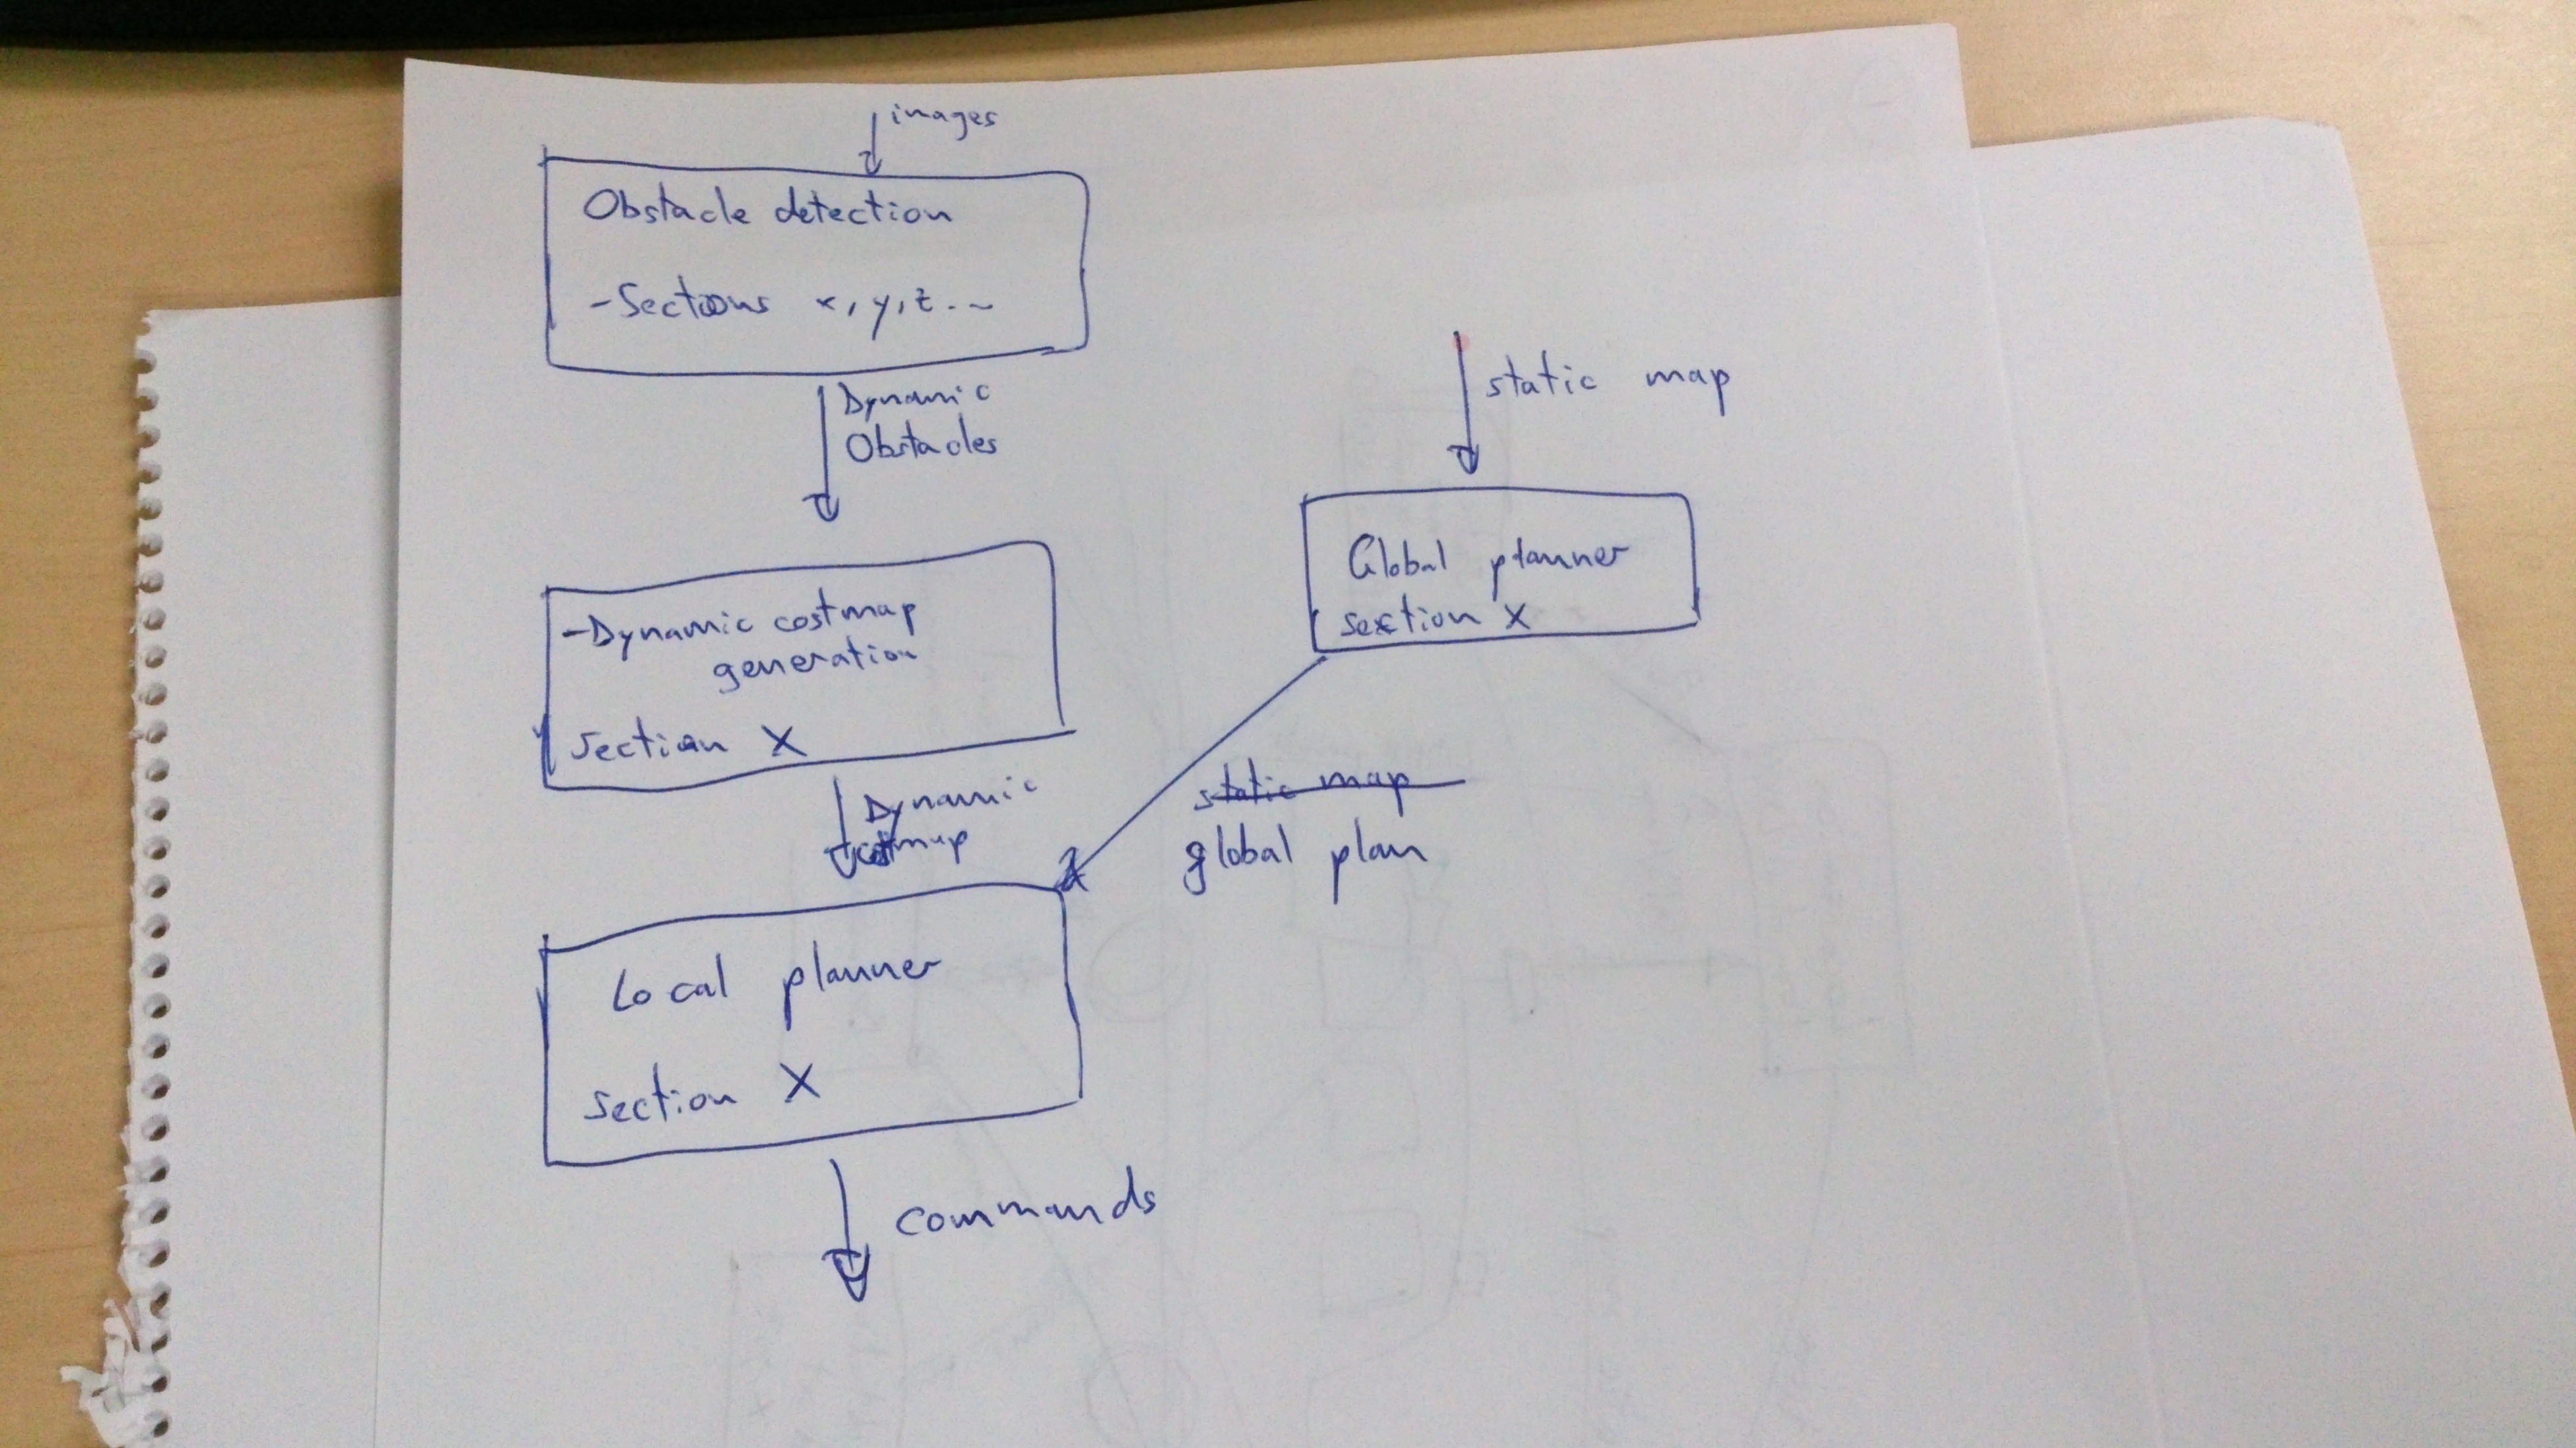
\includegraphics{pipeline}
  \caption{Pipeline of the modules described in this Thesis.}
\end{figure}

From the images captured in real-time, obstacles are located and passed to the module in charge of the generation of the dynamic costmap. At the same time, the static map is used for the generation of a feasible trajectory. Using the current position and vehicle status, the local planner tries to compute the proper commands in order to follow the global plan while trying to avoid the obstacles included in the dynamic costmap.

\section{Previous Work}\label{ch:chapter01_02}

Research on autonomous vehicles is a task being developed for a long time and for which a big effort has been carried on. A proof of that is the extensive literature existing about that topic, in special since the first of the DARPA Challenges (\cite{Buehler2007, Buehler2009}). Since then, the literature related to the topic has increased. Also, the interest on the use of Computer Vision in autonomous vehicles is growing, due to the possibilities that images offer when compared to other sensors, like \acp{LIDAR}.
In 1996, the ARGO project... \todo{Continuar desde aquí, una vez tenga una especie de historia de los vehiculos autonomos, en la intro.}
\todo{TerraMax, VIAC, Braive, Annieway y cualquier otro que pille por el camino.}
As depicted from section \ref{ch:chapter01_01}, the topics described in this thesis are quite diverse, so it is fair to review the state-of-the art of each of these topics separately.

\subsection{Change detection for obstacle localization in images}\label{ch:chapter01_02_01}

\todo{blah blah blah blah blah blah blah blah blah blah blah blah blah blah blah blah blah blah blah blah blah blah blah blah blah blah blah blah blah blah blah blah blah blah blah blah blah blah blah blah blah blah blah blah blah blah blah blah blah blah blah blah blah blah blah blah blah blah blah blah blah blah blah blah blah blah blah blah blah blah blah blah blah blah blah blah blah blah blah blah blah blah blah blah blah blah blah blah blah blah blah blah blah blah blah blah blah blah blah blah blah blah blah blah blah blah blah blah blah blah blah blah blah blah blah blah blah blah blah blah blah blah blah blah blah blah blah blah blah blah blah blah blah blah blah blah blah blah blah blah blah blah blah blah blah blah blah blah blah blah blah blah blah blah blah blah blah blah blah blah blah blah blah blah blah blah blah blah }

\subsection{Non-rigid point set registration for obstacle tracking}\label{ch:chapter01_02_02}

\todo{blah blah blah blah blah blah blah blah blah blah blah blah blah blah blah blah blah blah blah blah blah blah blah blah blah blah blah blah blah blah blah blah blah blah blah blah blah blah blah blah blah blah blah blah blah blah blah blah blah blah blah blah blah blah blah blah blah blah blah blah blah blah blah blah blah blah blah blah blah blah blah blah blah blah blah blah blah blah blah blah blah blah blah blah blah blah blah blah blah blah blah blah blah blah blah blah blah blah blah blah blah blah blah blah blah blah blah blah blah blah blah blah blah blah blah blah blah blah blah blah blah blah blah blah blah blah blah blah blah blah blah blah blah blah blah blah blah blah blah blah blah blah blah blah blah blah blah blah blah blah blah blah blah blah blah blah blah blah blah blah blah blah blah blah blah blah blah blah }

\subsection{Evaluation of stereo 3D reconstruction algorithms}\label{ch:chapter01_02_03}

\todo{blah blah blah blah blah blah blah blah blah blah blah blah blah blah blah blah blah blah blah blah blah blah blah blah blah blah blah blah blah blah blah blah blah blah blah blah blah blah blah blah blah blah blah blah blah blah blah blah blah blah blah blah blah blah blah blah blah blah blah blah blah blah blah blah blah blah blah blah blah blah blah blah blah blah blah blah blah blah blah blah blah blah blah blah blah blah blah blah blah blah blah blah blah blah blah blah blah blah blah blah blah blah blah blah blah blah blah blah blah blah blah blah blah blah blah blah blah blah blah blah blah blah blah blah blah blah blah blah blah blah blah blah blah blah blah blah blah blah blah blah blah blah blah blah blah blah blah blah blah blah blah blah blah blah blah blah blah blah blah blah blah blah blah blah blah blah blah blah }

\subsection{Stixel World}\label{ch:chapter01_02_04}

Apart from dense reconstruction algorithms, there are some methods that based on a stereo pair, are able to do a simplified reconstruction of the world. This reconstruction methods reject an important quantity of the information contained in the images, using just the information required for the avoidance of the obstacles. By doing so, a lot of computation time is saved. An example of this kind of algorithms is the work by \cite{badino2009stixel}, in which the world is represented through a set of ground-based vertical entities called stixels. The reconstruction of the stixels is based on the detection of the ground plane, and the stixels are grown from its basis up to the top of the detected obstacle. This allows avoiding the processing of the area of an image corresponding to the background. 
Based on this idea, some approaches have been taken. There are two main trends in the way in which stixels are computed. The main difference between them is the way in which the free space is computed. In \cite{pfeiffer2011towards, pfeiffer2013exploiting, pfeiffer2010efficient, muffert2012may}, this freespace computation is based on a disparity map and a probabilistic scheme is used in order to reduce the number of parameters. In they work, they assume that the number of objects captured along every column is small, there are not flying objects and the upper objects have a higher depths than the lower ones. In \cite{pfeiffer2013exploiting}, they improve the work presented in \cite{pfeiffer2011towards} by the use of three different stereo confidences, which are compared. In \cite{pfeiffer2010efficient}, they include a freespace computation scheme able to reduce the computational costs obtained for the previous works. They do a simple tracking and clustering of the stixels based on Kalman filters. Also, in \cite{muffert2012may} they compute the probabilities of a colission in a roundabout. There, the clustering is based on DBSCAN (\cite{ester1996density}) and freespace computation is based on a disparity map combined with B-splines \cite{wedel2009b}. 

The other research line based on stixels is based on the computation of the freespace without the need of disparity maps. It is the idea followed in \cite{benenson2011stixels, benenson2012pedestrian, benenson2012fast, gunyel2012stixels}, in which a very high frame rate is achieved by using a \ac{SAD} cube, with a value for each row, column and disparity combination. From this cube, the \emph{v}-disparity is computed and a model for the ground plane is obtained. Using the points in the boundary of the ground (obtained as a \ac{DP} problem), stixels are computed taking into account the height limitations of the expected obstacles and left-to-right occlusion constraints. 

\notsure{In section \todoref{XXX}, we introduce a method for the tracking of the stixels based on \cite{gunyel2012stixels}, in which we do the tracking of the stixels using bipartite graphs instead of \ac{DP}, as well as other metrics different from \ac{SAD}, obtaining better results both in terms of computation time and performance.}



% 
% 
% The first research line I've found is that followed by Benenson et al. [3,4,5]. They get a very huge frame rate (200 Hz in a CPU, 165 Hz when combined with a GPU objects detector). In this approach, there is no need to compute the SGM (or the chosen algorithm) for the whole image. This calculation is made with the use of a Sum of Absolute Differences cube, with a value for each row, column and disparity combination. Then, a model for the ground plane is obtained, which is linear, but can be changed by a nonlinear one. Using the points of the boundary in the ground, which is obtained as a DP problem, the stixels are obtained taking into account the limitations in height of the obstacles and left-to-right occlusion constraints. In this method, just one stixel is found by row.
% Advantages:
% It is fast and strong
% There is no need of obtaining a previous depth map
% The amount of data to be processed is highly reduced
% Uses (u,v) for stixel calculation, not just u
% Some examples in how to do classification
% Disadvantages:
% If ground plane detection fails, everything fails
% If matching costs are ambiguous or inaccurate, the height estimation fails
% Object height is restricted
% Flat ground plane used
% Just one stixel per column
% Just horizontal or vertical elements considered
% Parameter dependent (heigh constraint, for example)
% Some ideas related to this approach:
% Using a non-linear ground model
% Dynamic height
% More than one object per column
% Object detection
% Object “cleaning” (that is, for example in the case of pedestrians, we might have a silhouette of them instead of a square surrounding them)
% Making it able to process data from other sensors
% Tracking (Kalman or other method)
% Some “weird” ideas:
% Diagonal stixels
% J-Linkage or similar in order to detect several stixels (too expensive, however)
% 
% The other approach is that being followed in Daimler [6,7,8,9,10]. In this approach, they try to solve problems related to a bad calculation of the freespace area and try to reduce the number of parameters via a global probabilistic scheme. They assume that:
% the number of objects captured along every column is small.
% there are not flying objects.
% The upper objects have a higher depths than the lower ones.
% The initial version is that shown at [6]. Then, in [7] it is improved by using three different stereo confidences: Peak-ratio Naive, Maximum Likelihood and Local Curve. These are used to improve the results obtained by the global probabilistic scheme. Local Curve shows the best results. In [8], they include a freespace computation scheme in order to reduce computational costs, and they do a simple tracking and clustering of the stixels based on Kalman filters. Also, in [9] they compute if there will be a collision or not in a roundabout, but the stixel related approach is similar to that shown previously, except from the clustering, which is done using DBSCAN, being able to use both position and orientation; and also freespace computation is done based in B-splines. Times obtained are around 40 ms + the time for obtaining the depth map.
% In [10], the method is extended so they include existence estimation of the stixels, in order to avoid fake stixels in bad weather conditions.
% 
% Advantages:
% In the final versions, they use a free space computation, so the amount of data to be processed is reduced. But not as much as in the Benenson et al. work.
% A global probabilistic scheme
% Reduced parameterization
% Objects are allowed to be located at multiple depths
% Able to process data from other sensors as well
% Examples of how to track stixels and clustering
% Disadvantages:
% They need to obtain a depth map first
% Just horizontal or vertical elements considered
% Non-flying objects?
% There is not a cuantitative comparison with other methods other than theirs
% In tracking, stixels are not expected to move vertically
% Some ideas related to this approach:
% Use ELAS or ABBM instead of SGM, as they are faster and big quality is not so important (http://www.cvlibs.net/datasets/kitti/eval_stereo_flow_detail.php?benchmark=stereo&error=3&eval=all).
% Combine with Benenson approach.
% Object detection
% Object “cleaning” (that is, for example in the case of pedestrians, we might have a silhouette of them instead of a square surrounding them)
% Tracking (Kalman or other method)



\subsection{3D object tracking}\label{ch:chapter01_02_05}

By processing the data captured by sensors, it is desired to obtain the position, speed and size of an obstacle. However, usually sensors don't provide this information, so we need to process the information over time and do the tracking of detected obstacles. Many approaches that try to solve this problem, like \cite{danescu2012particle}, assume that obstacles have an standard geometry, and they are modeled as cuboids with associated position, size and speed vectors. This assumption is mostly correct in environments like highways, country roads, and certain urban scenarios, in which almost all the obstacles are cars, trucks or buses which can be simplified as cuboids. Also, these approaches tend to consider a flat ground.
However, this assumption cannot always done, as happens in pedestrian areas, intersections, off-road... In this case, we need to deal with specific shapes, sometimes with concave surfaces. The problem with this kind of obstacles is that methods that assume cuboid-shaped objects tend to wrap the obstacles with a convex shape, which causes an overestimation of their volume (\cite{broggi2013}). Another problem are those objects that are not laying on the ground, as happens with hanged traffic lights, tree crowns, lamps, etc. Usually, they are integrated into an occupancy grid as if they were touching the ground. About the ground plane assumption, in cases like that of an off-road scenario, it is important to estimate the real slope of the road in order to get good results.
Based on how much information they use, we can divide object tracking methods into two subcategories:
\begin{itemize}
 \item \emph{2.5D Solutions:} They do not make use of the complete information provided by 3D points. Instead of that, they tend to use elevation maps composed of uniform size cells. Each cell just stores occupancy and height information. This is the kind of methods that, as described before, usually consider obstacles as being in contact with a flat ground.
 In these methods, tracking is done before the complete reconstruction is done, in an intermediate point based on an specific feature. Based on this intermediate feature, we can distinguishing different kind of approaches:
  \begin{enumerate}
   \item \emph{Use of the 3D point as feature.} An example of this is the so called 6D vision (\cite{franke20056d}), in which the 3D stereo vision extracted information is combined with an efficient implementation of an optical flow in the image space based on a \ac{GPU}. Relevant points are tracked using a Kalman filter.
   \item \emph{Dynamic stixels.} This approach has been longer discussed in section \ref{ch:chapter01_02_04}. The 3D-situation is represented by a set of rectangular sticks named \emph{stixels}. Each stixel is defined by its 3D position relative to the camera and stands vertically on the ground, having a certain height.
   \item \emph{Tracked image features.} As example, check the work by \cite{barth2009estimating}. In this work, obstacles are represented as a rigid 3D point set which are tracked in terms of feature displacements and depth measurements.
   \item \emph{Sensor fusion.} \cite{wu2009collision} reconstruct the objects as cuboids from a stereo point cloud. In this process, position and speed values are improved to a very accurate value by the use of a radar along with stereo.
   \item \emph{Occupancy grids.} This is a very popular choice for tracking. An occupancy grid is a probabilistic map of the driving environment, which encodes the past and present knowledge from sensor data, and which can be updated dynamically when new information is available. These occupancy grids can be cartesian, with rectangular cells, polar, or even a relation between columns in an image an the disparity. An example of this is the method by \cite{danescu2012particle}, which has inspired part of the work described in section \todo { \ref{XXX}}.
   Another advantage of the model based on an occupancy grid is that it makes easier a collaborative update of the grid, which allows the usage of data from several sensors and observers.
  \end{enumerate} 
 \item \emph{3D Solutions:} Usually based on complex grid maps that use complete 3D information. Again, depending on how this grid is represented, we find 
 \begin{enumerate}
   \item \emph{Octree connected cubes.} An example is the work by \cite{wurm2010octomap} or \cite{broggi2013}.
   \item \emph{Adjacent stacks of cells}, as described in \cite{Moravec96robotspatial} 
 \end{enumerate}
\end{itemize}

\subsection{Global planning}\label{ch:chapter01_02_06}

% Muchos estudios se han realizado en torno al problema de generacion de rutas globales. Aunque fue inicialmente propuesta para aplicaciones en robotica, ultimamente se ha usado con exito en aplicaciones de automocion.
% 
% Podemos dividir los algoritmos de planificacion en... (El resto esta en la libreta, en la parte de estado del arte de planificacion local)
% 
% 
% Los algoritmos de planificacion pueden ser divididos en locales y globales:
% Globales:
%   La ruta global y los estados del vehiculo quedan determinados por la info proporcionada por un mapa digital y un sistema de localizacion
% Locales:
%   La ruta local puede ser generada entonces en la etapa de planificacion basada en la ruta global y la info del entorno del vehiculo obtenida por los sensores
%   El paper se basa en local path planning que proporciona capacidades de evitacion de obstaculos a un vehiculo autonomo que sigue una ruta global predefinida

% Hablar de las bandadas de pájaros


\subsection{Local planning}\label{ch:chapter01_02_03}

With a generated path, there problem is computing the commands that the vehicle needs in order to follow that path while avoiding the occasional obstacles in the way of the vehicle. In the literature, many methods are based in searching a set of trajectories that act as intermediaries between this global path and the local path, all of them starting from the vehicle and evolving in time following an specific model, most of them following a discrete optimization scheme (\cite{thrun2006stanley, montemerlo2008junior, werling2010optimal, ferguson2008motion}).
Sampling based approaches are suitable for planning problems in the high dimensional space. The algorithm builds a collision-free path from the initial configuration to the goal path. The configuration that defines the position and orientation of the vehicle is sampled. From all the approaches of this kind, \ac{RRT} and its variants are widely used in non-holonomic motion planning applications.
\acp{RRT} are incrementally built in a way in which that the estimated distance from an specific point to the tree is quickly reduced. However, for real time implementations require efficient heuristics for the sampling configuration. 
Some examples of this kind of methods are \cite{van1997real}, \cite{lavalle2001randomized} and \cite{kuwata2009real}.

These methods compute a finite set of trajectories based on a parametric model, usually polynomial functions of a given order, The problem with this is that, despite of the fact that the space of possible solutions is reduced, allowing a efficient planning, can introduce suboptimality, reaching to overshoots or stationary offsets in curves.
Some other methods, which are inside the discrete optimization approaches, are based in the transformation of the configuration space through the Fren\'et space. Some examples are these:
\begin{itemize}
 \item In \cite{werling2010optimal}, long term objectives are performed, like speed keeping, merging, following, stopping. This is done through optimal control strategies within the Fren\'et frame of the street.
 \item In \cite{thrun2006stanley}, lateral offset is defined as the perpendicular to a established base trajectory. This allows the vehicle to drive along the road parallel to this trajectory. In order to select the optimal path, the cost function penalizes passing over obstacles and the distance respect to the center of the current road.
 \item In \cite{chu2012local}, also a set of candidate paths are generated, with endpoints in fixed positions at different offsets respect to the base frame, but they do not set this base frame in the center of the road, as it could be dangerous when computing the costs at certain scenarios. Instead of that, they use a security cost for each candidate path. Security of the path is computed by blurring the binary data of the obstacles. They also have into account certain criteria, as the smoothness cost or the path consistency between iterations.
\end{itemize}

\section{Summary}\label{ch:chapter01_03}

In this chapter, we have described a general idea of the work presented in this Thesis. Also, the pipeline of the final developed application is introduced. All this information will be explained in more detail in the following sections, including implementation details together with some results and a discussion of the advantages/disadvantages of the different methods.

